\documentclass[a4paper,12pt]{report}
\usepackage[utf8]{inputenc}

\title{Report}
\author{Rocco Caruso}
\usepackage{fancyhdr} 
\usepackage{url} % per scrivere gli indirizzi Internet
\usepackage{hyperref}
\usepackage{amsthm}
\usepackage{amsmath}
\usepackage{graphicx} %per le immagini
\usepackage{wrapfig}
\usepackage{caption}
\usepackage{subcaption}
\usepackage[
backend=biber,
style=alphabetic,
sorting=ynt
]{biblatex}
 \addbibresource{bib.bib}
\begin{document}
%comandi per teoremi ed enunciati
\theoremstyle{definition}
\newtheorem{definizione}{Definizione}
\newtheorem{teorema}{Teorema}
\maketitle
\graphicspath{ {./immagini/} }%path alla cartella immagini
\chapter{Problem definition}
 
Dato uno stream  di tweet (ordinato temporalmente) l’obiettivo  è quello di individuare dei "topic” o “event”. In letteratura esistono due principali metodologie: 
\begin{itemize}
\item document-pivot
\item feature-pivot
\end{itemize}
In questo lavoro è stata adottata la prima metodologia, l'obiettivo è quindi suddividere lo stream in cluster, tali che ciascun cluster corrisponda a tutti i tweet relativi ad un “evento “. E’ altresì necessario, una volta suddiviso lo stream in vari cluster, distinguere quali sono realmente eventi (flashmob) da quelli che non lo sono, per mezzo di un classificatore. \\
La definizione di evento utilizzata è quella utilizzata per il Topic Detection and Tracking (TDT) \cite{Allan:2002:TDT:772260} :
\begin{definizione}
\label{def:event}
\textit{un evento è qualcosa che accade in un luogo specifico in un tempo specifico}
\end{definizione}
L’intero processo può essere suddiviso in 5 attività come descritto in figura \ref{fig:workflow} 

\begin{figure}[h]
    \centering
    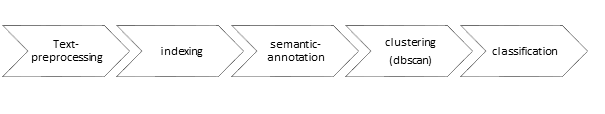
\includegraphics[width=0.8\textwidth]{workFlow}
    \caption{workflow}
    \label{fig:workflow}
\end{figure}  



\newpage 
 
\section{Preprocessing}
Il preprocessing è uno step essenziale per qualunque task di text-mining, quando si ha a che fare con testo derivante dai social media come twitter, tale step diviene di vitale importanza a causa delle caratteristiche dei tweet.
\`E dunque necessaria una fase accurata di preprocessing per il testo dei tweet prima di poter eseguire qualsiasi modellazione su di essi. Il primo passo in questa fase è la rimozione di quelle feature testuali legate ai tweet come:
\begin{itemize}
\item \emph{url:} dal testo sono eliminati tutti i riferimenti a url o media  
\item \emph{@-mentions:} vengono eliminate tutte le mentions ad altri utenti
\item  \emph{\#hashtag:} Per quanto riguarda gli hashtag viene solo eliminato il caratattere   \#   poich\`e se fossero eliminati si potrebbe perdere della semantica dal testo.
Inoltre spesso nei tweet gli hashtag sono composizioni di più parole dove ciascuna parola inizia con una lettera maiuscola (camel Case), come ad esempio \#StopBombingGaza. Gli hashtag che si presentano nella forma su descritta verranno scomposti in nelle parole che di cui sono composti (\#StopBombingGaza $\rightarrow$ Stop Bombing Gaza).
\item \emph{RT:} per i retweet viene considerato il testo del tweet originale.
\end{itemize}
Per il primo passo non è necessaria alcuna fase di parsing del testo poich\`e tutte queste informazioni sono fornite dalle api di twitter sotto forma di dati strutturati\footnote{nell attributo entities del tweet}. Molto spesso i tweet sono composti da keywords appartenenti a lingue diverse o contengono caratteri speciali, per tale motivo saranno eliminati tutti i non latin characters. Tramite apposita espressione regolare vengono identificati ed eliminate le emoticons presenti nel testo. Una volta effettuate queste pulizie, si passa all’identificazione della lingua del tweet per mezzo di una libreria java\footnote{https://code.google.com/p/language-detection/}, e saranno considerati solo i tweet in lingua inglese.
\newpage

\section{Indexing} 
Il testo del tweet verrà rappresentato con un boosted tf-idf vector utilizzando Apache-lucene\footnote{\href{https://lucene.apache.org/core/}{https://lucene.apache.org/core/}}. 
A partire dal testo dei tweet ripulito, sono state effettuati ulteriori step di nlp come :
\begin{itemize}
\item stop word removal
\item pos tagging (tramite lo stanford pos tagger addestrato su un modello  creato a partire da tweet
\item stemming (o lemmtization)
\end{itemize}
Poich\`e si analizza uno stream di tweet in maniera incrementale è necessario che anche lo schema di pesatura tf-idf sia incrementale ovvero le document-frequencies per una word $w$ variano nel tempo. 

Il peso di una word $w$ di un tweet avente tempo $t$ è dato da:
\begin{equation}
tf-idf_w=tf(w)\ log\frac{N_t}{df_t(w)}boost(w)
\end{equation}
Dove $N_t$ è il numero di tweet al tempo $t$.
Risulta fondamentale assegnare un boost a determinate word poiché, a causa della natura dei tweet (max 140 caratteri), il $tf$ di ciascuna keyword è solitamente pari a 1.  


\begin{equation*}
boost(w):=\begin{cases}
2.0 & \text{se $w$ è un hashtag,}\\
1.5 & \text{se $w$ è un Proper-Noun,}\\
1& \text{altrimenti.}
\end{cases}
\end{equation*}
Solitamente uh hashtag ha un alto potere informativo all’interno di un tweet, nel lavoro di  Phuvipadawat \cite{Phuvipadawat:2010:BND:1913791.1913911}  il boost pari a 1.5  per i poper-noun ha prodotto risultati migliori.

\newpage
\section{Semantic Annotation}
Tramite Dbpedia-Spootlight \cite{isem2013daiber} è possibile annotare automaticamente il testo dei tweet con DBpedia URIs.  Ciò permette di arricchire la rappresentazione testuale andando a lenire i classici problemi di ambiguità del linguaggio naturale come polisemia e sinonimia.  
Annotare il testo con DBpedia URis permette di sfruttare la base di conoscenza di DBpedia per poter determinare la correlazione semantica fra due termini. 
Il progetto DBpedia \cite{DBLP:conf/semweb/AuerBKLCI07} oltre a organizzare in maniera strutturata le informazioni di Wikipedia, le collega ad ulteriori open-datasets come: US Census, Geonames, MusicBrainz, the DBLP bibliography, WordNet, Cyc, tramite RDF links come mostrato in figura \ref{fig:dbpedia}  
\begin{figure}[h]
    \centering
    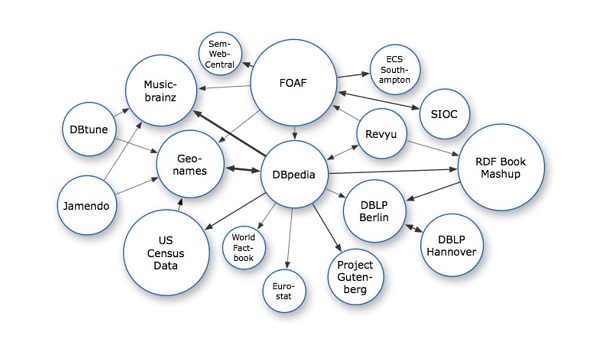
\includegraphics[width=0.6\textwidth]{dbpedia}
    \caption{Datsets interconnessi a DBpedia.}
    \label{fig:dbpedia}
\end{figure}  

Avendo due risorse DBpedia è possibile definire una funzione di distanza, che sfrutti la base di conoscenza di DBpedia. \`E stata definita  una funzione di distanza \emph{Dbpedia Semantic Distance DSD}, che impiega sia DBpedia che il dataset geografico Geonames per risorse di tipo geografico, come segue:
\begin{equation} \label{eq:dbpedia_semantic_distance}
DSD(a,b):=\begin{cases}
GeoDist(a,b) & \text{se $type(a)=location \land type(b)=location$  ,}\\
NDD(a,b) & \text{altrimenti}\\
\end{cases}
\end{equation}
Dove $DSD(a,b) \in [0,1]$,
Milne e Witten \cite{Milne08aneffective} hanno utilizzato gli hyperlink delle pagine Wikipedia per poter definire la correlazione fra due articoli wikipedia (e quindi due risorse dbpedia): date due risorse $a,b$, possiamo definire una \emph{Normalized DBpedia Distance (NDD)} come segue:
\begin{equation} \label{eq:normalized_dbpedia_distance}
NDD(a,b):=\begin{cases}
\frac{\log(max\{|A|,|B|\})-log( |A \cap B|\})}{N-\log(min\{|A|,|B|\})} & \text{se $A \cap B \neq \emptyset $  ,}\\
1 & \text{altrimenti}\\
\end{cases}
\end{equation}
 $A$ e $B$  sono gli insiemi delle risorse DBpedia che hanno un link rispettivamente verso $a$ e $b$, mentre $N$ è il numero totale di risorse in DBpedia. Questa distanza varia nell'intervallo [0,1] dove 1 sta ad indicare che non vi è nessuna correlazione fra i due concetti, mentre 0 indica che i due concetti hanno lo stesso significato. L'idea alla base, è che due risorse saranno simili se esiste una terza che ha un link verso entrambe.
 
Per le risorse DBpedia di tipo "location"\footnote{per risorse di tipo location si intendono quelle risorse classficate come http://dbpedia.org/ontology/Location} è stata definita la funzione di distanza  \ref{eq:geoDistance} che impiega il dataset "GeoNames". Poiché il task, è quello di identificare eventi\ref{def:event} che accadono in un luogo specifico, è utile valutare la correlazione sulla base di informazioni geografiche. Geonames \footnote{\href{http://www.geonames.org/}{http://www.geonames.org/}} è un database geografico contenente più di 10 milioni di nomi geografici, ogni risorsa è classificata  da una “feature class”  (administrative divisions, populated places, structures, mountains, water bodies, etc) e ulteriormente sotto classificata da 645 “feature codes”. Tra le varie informazione e relazioni che interconnettono le risorse nell'ontologia sono state utilizzate le seguenti per poter valutare la similarità fra le risorse:
\begin{itemize}
\item \emph{Country-code:} codice identificativo della nazione cui appartiene la risorsa
\item \emph{FeatureClass}
\item \emph{FeatureCode} 
\item \emph{parentADM1:} risorsa di tipo ADM1(regione) che contiene la risorsa
\item \emph{parentADM2:}  risorsa di tipo ADM2(provincia) che contiene la risorsa
\item\emph{Coordinates:} (latitude,longitude)

\end{itemize}
La funzione di similarità deve quindi tener conto dei diversi livelli di granularità delle risorse Geonames e sfruttare le relazioni fra di esse. Verrà definita una distanza \emph{Geonames Distance (GD)} compresa fra [0,1] cosi definita:
\begin{equation}
\label{eq:geonamedistance}
GD(a,b):=\begin{cases}
0.8 & \text{se $\exists c \;| \;(c\; parentADM1 \;a)\; \land \; (c\; parentADM1 \;b) $}\\
0.8 & \text{se  $ \:\:(a\; parentADM2 \;b)\; \lor \; (b\; parentADM2 \;a) $}\\
0.3 & \text{se $\exists c \;| \;(c\; parentADM2 \;a)\; \land \; (c\; parentADM1 \;b) $}\\
0.3 & \text{se  $ \:\:(a\; parentADM2 \;b)\; \lor \; (b\; parentADM1 \;a) $}\\
1& \text{altrimenti.}
\end{cases}
\end{equation}
Per alcune risorse di granularità più fine come città, parchi, edifici ha senso invece, considerare le coordinate. Avendo le coordinate è possibile calcolare la distanza espressa in km fra di esse usando l’Harvesine Forula\footnote{Haversine formula}.Sia $d$ la distanza espressa in km tra $a$ e $b$, verrà definita una \emph{Coordinate Distance (CoordDist)} 
\begin{equation}
\label{eq:coordinatedistance}
coordDist(a,b):=\begin{cases}
0.0 & \text{se $0<d\leq5$,}\\
0.2 & \text{se $5<d\leq10$,}\\
0.25 & \text{se $10<d\leq15$,}\\
0.3 & \text{se $15<d\leq25$,}\\
0.4 & \text{se $25<d\leq40$,}\\
0.7 & \text{se $40<d\leq50$,}\\
0.8 & \text{se $70<d\leq80$,}\\
1& \text{altrimenti.}
\end{cases}
\end{equation}
Si può cosi definire la distanza geografica \emph{GeoDist} come segue:
\begin{equation}
\label{eq:geoDistance}
GeoDist(a,b):=\begin{cases}
coordDist(a,b)& \text{se sia a e b hanno coordinate}\\
GD(a,b)&  \text{altrimenti.}
\end{cases}
\end{equation}

\newpage
\section{Clustering}
L'algoritmo di clustering utilizzato è Incremental Dbscan poiché può gestire bene il rumore e non necessita di parametri come il numero di cluster a priori. La distanza utilizzata si basa sia sulla rappresentazione tf-idf del tweet sia sui DBpedia URIs estratti :
\begin{equation}
dist(a,b)=1- timeSim(a,b)\,\frac{textSim(a,b)+semanticSim(a,b)}{2}
\end{equation}
La similarità testuale è data dalla similarità del coseno fra i vettori tf-idf dei due tweet:
\begin{equation*}
textSim(a,b)=\frac{v_a \cdot  v_b}{||v_a||\:||v_b||}
\end{equation*}
 Anche il tempo di creazione dei tweet verrà preso in considerazione per valutarne la distanza, poiché anche se due tweet avessero un testo molto simile es \emph{“tonight  flashmob in central park”}, ma fossero pubblicati ad un mese di distanza, è molto inverosimile che si riferiscano al medesimo evento. Per tale ragione, è stata definita una similarità temporale  \footnote{d$_a$=\#days from the epoch of tweet $a$}
\begin{equation*} 
timeSim(a,b):=\begin{cases}
1-\frac{|d_a-d_b|}{31} & \text{se $|d_a-d_b|<31 $  ,}\\
0 & \text{altrimenti}\\
\end{cases}
\end{equation*}
Ad un tweet, tramite il processo di annotazione semantica, possono essere associate una nessuna o più risorse DBpedia,la distanza semantica sarà data dalla distanza degli insiemi di risorse associati ai due tweet valutata secondo la distanza definita in precedenza per le risorse DBpedia\ref{eq:dbpedia_semantic_distance}. La similarità fra un elemento $x$ e un insieme $Y$ è data da:
\begin{equation*}
	sim(x,Y)=sup\{1-DSD(x,y)\:| y\in Y \}
\end{equation*}

Dati due insiemi di risorse DBpedia $D_a,D_b$ la similarità fra i due insiemi sarà definita come: 
\begin{equation}
sim(D_a,D_b)=\frac{\sum\limits_{x \in D_a} sim(x,D_b)  }{|D_a|} 
\end{equation}

Questa funzione di similarità non è simmetrica,\footnote{se $D_a\subseteq D_b\Rightarrow sim(D_a,D_b)\neq sim(D_b,D_a) $}
Per ottenere una funzione simmetrica è sufficiente definirla come: 
\begin{equation*} 
semanticSim(a,b):= 
\begin{cases}
\frac{sim(D_a,D_b)+sim(D_b,D_a)}{2} & \text{se $D_a,D_b\neq \emptyset$ }\\
1& \text{altrimenti.}

\end{cases}
\end{equation*}
Se ad uno dei due tweet non è associata nessuna risorsa, la similarità semantica sarà pari ad uno, quindi la loro similarità sarà valutata  solo in base alla loro rappresentazione testuale.
Utilizzare una similarità semantica serve ad attenuare il problema della “fragmentation” di cui sono affetti i metodi document-pivot, ovvero utilizzando solo la similarità testuale molti eventi possono essere erroneamente suddivisi in più cluster.  Inoltre Petkos e Papadopoulus \cite{DBLP:conf/www/PetkosPK14}  hanno constato che se due tweet condividono uno stesso URL, o  un tweet e in reply all’altro, allora si riferiscono allo stesso topic/evento.
 
\begin{figure}
    \centering
    \begin{subfigure}[b]{0.45\textwidth}
        \centering
        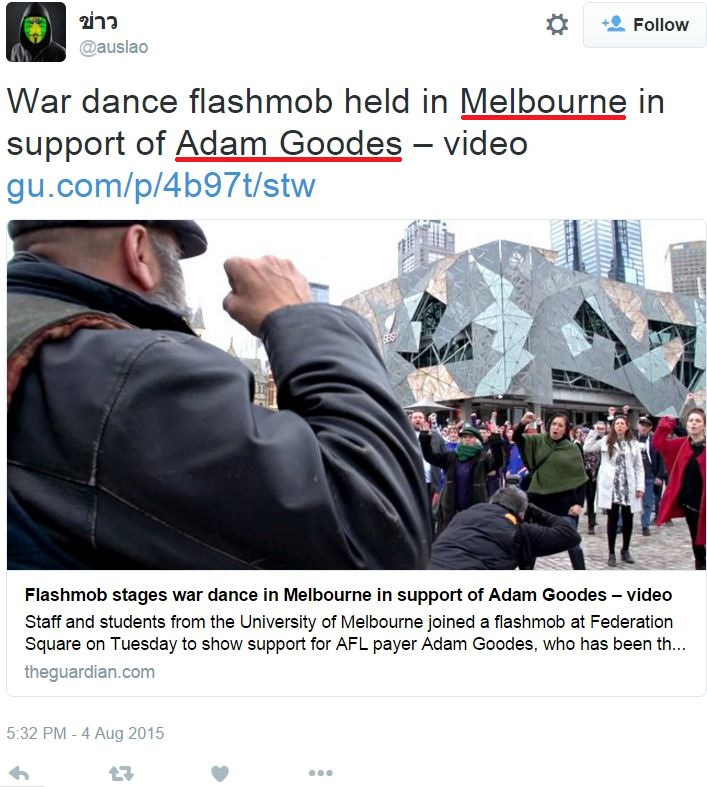
\includegraphics[width=\textwidth]{tweetA}
        \caption{}
        \label{fig:tweeta}
    \end{subfigure}
    \hfill
    \begin{subfigure}[b]{0.45\textwidth}
        \centering
        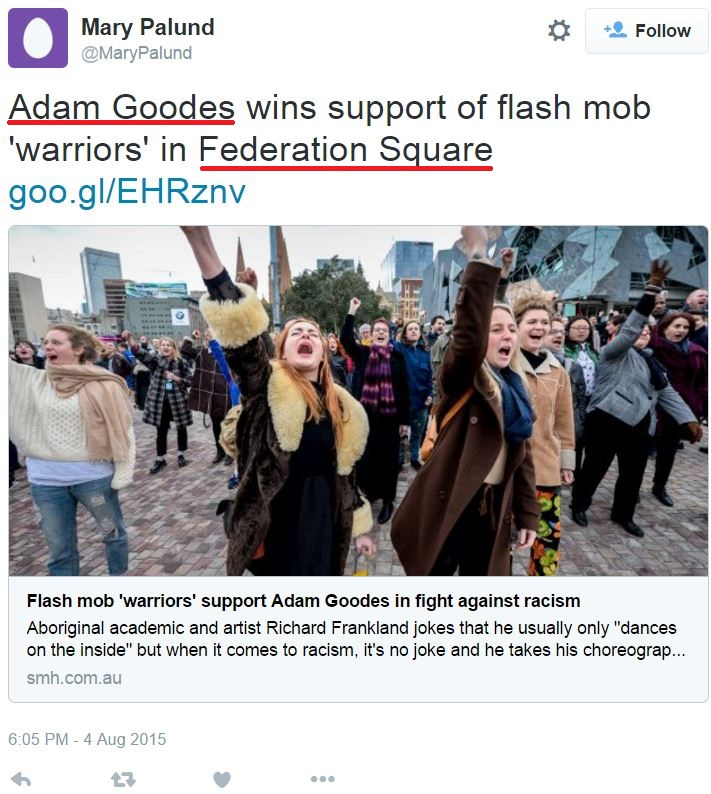
\includegraphics[width=\textwidth]{tweetB}
       \caption{}
        \label{fig:tweetb}
    \end{subfigure}
    \hfill
    
    \caption{Due tweet appartenti allo stesso cluster}
    \label{fig:twotweets}
\end{figure} 
Si considerino i tweet $a,b$ in figura \ref{fig:twotweets}:

\begin{itemize}
\item $textSim(a,b)=0.46$ 
\item $timeSim(a,b)=1.0$ i tweet sono stati pubblicati entrambi il 4/8/2015
\item $semanticSim(a,b):=\frac{sim(D_a,D_b)+sim(D_b,D_a)}{2} $



  $D_a=$\{ \textless\href{http://dbpedia.org/resource/Melbourne}{Melbourne}\textgreater, \textless\href{http://dbpedia.org/resource/Adam_Goodes}{Adam Goodes}\textgreater\}
  
  $D_b=$\{ \textless\href{http://dbpedia.org/resource/Adam_Goodes}{Adam Goodes}\textgreater, \textless\href{http://dbpedia.org/resource/Federation_Square}{Federation Square}\textgreater\}
  
\begin{align*}
 NSD(Melbourne,Adam Goodes)&=NDD(Melbourne,Adam Goodes)\\
 &= \frac{\log(max\{|A|,|B|\})-log(|A \cap B|)}{N-\log(min\{|A|,|B|\})}\\
 &= \frac{\log(643)-log(10)}{N-\log(138)}=0.367  
\end{align*} 
\begin{align*}
 NSD(Melbourne,Federation Square)&=\\
 =GeoDist(Melbourne,Federation Square)&=\\
 =CoordDist(Melbourne,Federation Square) &=0 \: \text{(poichè la distanza in km è 0.8)}
\end{align*}  
\begin{align*}
 NSD(Adam Goodes,Federation Square)=&\\
 NDD(Adam Goodes,Federation Square)&=1 \: \text{poichè} \: A \cap B=\emptyset
\end{align*} 

\begin{align*}
 sim(Melbourne,D_b)&=sup\{1-DSD(Melbourne,y)\:| y\in D_b \}\\
	&=sup\{(1-DSD(Melbourne,Adam Goodes)),\\
	&\:\:\:\:(1-DSD(Melbourne,Federation Square))\}\\
	&=sup\{(1-0.367),(1-0)\}=1	\\	  
 sim(Adam Goodes,D_b)&=sup\{1-DSD(Adam Goodes,y)\:| y\in D_b \}\\
	&=sup\{(1-DSD(Adam Goodes,Adam Goodes)),\\
	&\:\:\:\:(1-DSD(Adam Goodes,Federation Square))\}\\
	&=sup\{(1-0),(1-1)\}=1\\		 
sim(D_a,D_b) &=\frac{1+1}{2}=1 ,\: sim(D_b,D_a) :=\frac{1+1}{2}=1\\
&\implies semanticSim(a,b)=1
\end{align*}
\end{itemize} 
 \begin{align*}
dist(a,b)&=1- timeSim(a,b)\,\frac{textSim(a,b)+semanticSim(a,b)}{2}\\
&=1-\frac{0.46+1}{2}=0.269
\end{align*}

Se invece, $SemanticSim$ fosse definita come la media delle distanze fra tutte le possibili coppie fra i due insiemi avremmo: 

\begin{align*}
	semanticSim(a,b)&=\frac{\sum\limits_{x \in D_a} \sum\limits_{x \in D_b}  (1-NSD(x,y))}{|D_a||D_b|}=\\
	&=\frac{(1-0.36)+(1-0)+(1-0)+(1-1)}{4}=0.73
\end{align*}
  
 
 


\newpage
\section{Classification}
Per poter filtrare gli eventi reali da quelli non reali è stato addestrato un classificatore SVM, sulla base di statistiche derivanti da cluster individuati. Tali statistiche derivano da feature dei tweet che compongono i cluster e dalle annotazioni estratte da tali tweets.
\begin{itemize}
\item TWEET FEATURES
\begin{itemize}
	\item	\%retweets:  percentuale di retweets presenti nel cluster. 
\item	\%replies:      percentuale di tweet nel cluster che sono replies
\item	\%mentions: percentuale di tweet nel cluster che contengono mentions
\item	\%hashtags:  percentuale di tweet nel cluster che contengono hashtag
\item	\%urls: percentuale di tweet nel cluster che contengono urls
\item	\%media: percentuale di tweet nel cluster che contengono media
\item	\%authors: percentuale di autori distinti dei tweet nel cluster (se i tweet sono stati creati 
\end{itemize}
\item TOPIC FEATURES
\begin{itemize}
\item avg token number: numero medio di token dei tweet che compongono il cluster
\item \%WhereAnnotations: percentuale di tweet nel cluster che contengono annotazioni semantiche di tipo Location
\item HasSpecificLocation: booleano che indica se fra le annotazioni di tipo location vi sia almeno una con delle coordinate specifiche.
\end{itemize}
\end{itemize}

\chapter{dbpedia}
Wikipedia \footnote{https://en.wikipedia.org/} è divenuta una delle maggiori risorse di conoscenza disponibili nel web, ed è manutenuta da migliaia di utenti (collaboratori). Gli articoli Wikipedia sebbene composti prevalentemente da testo, contengono informazioni semi-strutturate come: template infobox , informazioni sulla categorizzazione dell'articolo, immagini, geo-coordinate e link sia verso altre pagine web sia verso altre pagine wikipedia.
Gli infobox sono tabelle di coppie attributo valore, che mostrano i dati più rilevanti di ciascuna pagina wikipedia. Il progetto DBpedia \cite{Bizer:2009:DCP:1640541.1640848} estrae dati strutturati da wikipedia tramite un extraction framweork open source e li unisce in una base di conoscenza multi dominio e multi lingua. Per ogni pagina presente in wikipedia, viene associato un \emph{Uniform Resource Identifier (URI)} in DBpedia per identificare un'entità o un concetto descritto dalla corrispondente pagina Wikipedia della versione inglese. Durante il processo di trasformazione, i dati semi-strutturati come i campi infobox,categorie, pagelinks sono convertiti in triple RDF e aggiunte alla base di conoscenza come proprietà dell'entità identificata dall URI.  Per rendere omogenea la descrizione delle informazioni, è stata sviluppata un ontologia e sono state definite le corrispondenze fra le proprietà presenti negli infobox e l'ontologia.
L'ontologia DBpedia consisite di 320 classi e descritte da 1650 proprietà. Le classi organizzate mediante una gerarchia sussuntiva dove \emph{owl:Thing} è la classe più generale. Poiché Il sistema di Wikipedia infobox si è evoluto in maniera decentrata, talvolta accade ad esempio che si usino diversi template per la stessa tipologia di entità (class) o si usino nomi diversi per descrive lo stesso attributo (es placeOfBirth o birthPlace). 
 L'allineamento tra i template infobox e l'ontologia a causa di queste eterogeneità presenti nella nomenclatura, non è quindi completamente automatico, ma si basa anche su mapping definiti manualmente, forniti dalla comunità di DBpedia. Ad esempio ‘date of birth’ and ‘birth
date’ sono entrambi mappati con la proprietà birthDate. 
\subsection{Accedere a DBpedia}
La base di conoscenza DBpedia è disponibile sul web sotto GNU Free Documentation, e può essere consultata mediante varie modalità :
\begin{itemize}
\item \emph{Linked Data: linked data è la metodologia di pubblicazione  dei dati RDF nel web, che utilizza gli URI http come identificativo delle risorse e il protocollo HTTP per ritrovare al descrizione rdf delle risorse. Quando si accedere ad un URI di una risorsa DBPedia mediante un semantic web agent si ottiene la descrizione rdf della risorsa mentre se si utilizza un semplice web-browser si otterrà una vista html descrizione.
} 
\item \emph{Sparql Endpoint } \'E fornito un endopoint mediante il quale si può interrogare la base di conoscenza tramite il protocollo SPARQL.
\item \emph{RDF dumps} la base di conoscenza è stata suddivisa in varie parti in base agli rdf-predicate 
\end{itemize}

 
\chapter{Stato dell'Arte} 
\section{Event detection nei media tradizionali}
L'attività di event-detection è stata a lungo utilizzata per individuare eventi da stream testuali derivanti dai media più tradizionali come giornali o radio, infatti l'event-detection è stata per molto tempo oggetto di ricerca del programma di \emph{Topic Detection and Tracking TDT} \parencite{All02}, un' iniziativa	promossa dalla DARPA \footnote{Agenzia di ricerca agenzia per i progetti di ricerca avanzata per la difesa}, con lo scopo di organizzare stream di notizie testuali sulla base degli eventi di cui discutono. Secondo il TDT, l'obiettivo dell'attività di \emph{event detection}, è scoprire nuovi  eventi o eventi precedentemente non noti, a partire da stream di notizie testuali derivanti dai media tradizionali come notiziari o newswire, dove ciascun evento si riferisce ad un \emph{qualcosa, non banale, che accade in un luogo e tempo specifico}. Le tecniche di event-detection possono essere classificate in due macro categorie: \emph{document-piovot} e \emph{document piovot} a seconda che utilizzino feature dei documenti o feature temporali delle singole keywords presenti nei documenti. 
La prima scopre eventi effettuando un clustering dei documenti sulla base di una qualche funzione di distanza fra i documenti stessi \cite{Yang:1998:SRO:290941.290953}, mentre nella seconda si studia la distribuzione delle singole parole e scoprono nuovi eventi raggruppando le parole \cite{Kleinberg:2002:BHS:775047.775061} 
Come evidenziato da \cite{Yang:1998:SRO:290941.290953} infatti, l'event detection può essere ricondotto al problema della scoperta di pattern in uno stream testuale, quindi il modo più naturale per scoprire nuovi eventi, è quello di usare un algoritmo di clustering. Il task di event-detection si può suddividere in tre fasi principali: data preprocessing, data rappresentation, data organization o clustering. Nella fase di preprocessing in questa fase vengono applicate al testo delle classiche tecniche di NLP come la rimozione di stopwords, tokenizzazione e stemming.
I modelli di rappresentazione di dati più utilizzati per l'event detection sono  \emph{il modello vettoriale} e  \emph{i modello bag of words}, i cui elementi saranno diversi da zero, se il termine corrispondente è presente nel documento. A ciascun termine nel vettore, è assegnato un peso secondo lo schema \emph{tf-idf}\cite{Salton:1989:ATP:77013} che valuta quanto è importante una parola per un documento all'interno di un corpus. Questo modello di rappresentazione non prende in considerazione l'ordine temporale delle parole ne caratteristiche sintattiche o semantiche del testo come il part of speech tag o named entities. Per questa ragione utilizzando questo modello, ad esempio, sarebbe difficile distinguere due eventi simili ma accaduti ad un mese di distanza fra loro. Nel lavoro di \cite{Yang:1998:SRO:290941.290953} il task di scoperta di nuovi eventi da uno stream testuale di news è suddiviso in due fasi principali:
Retrospective Event Detection (RED), New Event Detection (NED). La prima fase (RED) comporta la scoperta di eventi da una collezione già nota di documenti, mentre nella seconda si cerca di identificare gli eventi dallo stream di notizie in tempo reale. Per il RED è stato utilizzato un algoritmo di clustering gerarchico: \emph{Group Average Clustering GAC}, che consente anche di descrivere gli eventi identificati con diversi livelli di granularità. Per la fase di New Event Detection, invece, solitamente viene adottato un agoritmo di clustering incrementale single-pass \cite{Allan:2002:TDT:772260,Yang:1998:SRO:290941.290953} che consente di suddividere i documenti nei vari cluster non appena arrivano dallo stream. In particolare ciascun documento viene elaborato sequenzialmente e viene assorbito dal cluster più simile, o verrà creato un nuovo cluster se la similarità è al di sotto di una soglia prestabilita. In un ambiente di detection on-line (NED) un forte vincolo è costituito dal fatto che non si può hanno informazioni di eventi futuri,ovvero non è possibile utilizzare dati provenienti da documenti successivi, cronologicamente, a quello corrente. Utilizzando un modello di rappresentazione vettoriale, questo vincolo pone delle problematiche su come gestire la crescita del vocabolario dei termini quando vengono aggiunti nuovi documenti al corpus e come modificare delle statistiche inerenti l'intero corpus come l'IDF. La soluzione suggerita da  \cite{Yang:1998:SRO:290941.290953} è quella di modificare il vocabolario dei termini in maniera incrementale e modificare l'IDF ogni qual volta viene aggiunto un nuovo documento. 
\begin{equation}
\label{eq:incIDF}
idf_t(w)=log_2 \left(\frac{N_t}{df_t(w)} \right) 
\end{equation}
dove $N_t$ è il numero di documenti fino al tempo $t$ e $df_t(w)$ è la document frequency della keyword $w$ fino al tempo $t$.
In pratica questi approcci NED, tendono a divenire molto costosi sia in termini di risorse computazionali che di tempo richiesto, e in taluni casi addirittura irrealizzabili se non utilizzando delle tecniche che ne migliorino l'efficienza. Una possibile tecnica per ridurre i costi è quella di utilizzare una \emph{slidining time window} \cite{Luo:2007:RRN:1247480.1247536,Papka:1999:ONE:897559} per limitare il numero vecchi documenti da analizzare quando si prende in considerazione un nuovo documento. Utilizzare una finestra temporale non solo riduce i costi, ma rende possibile di limitare lo scope degli eventi scoperti, permettendo di identificare eventi simili ma che accadono in uno slot temporale diverso \cite{Yang:1998:SRO:290941.290953}. Tutte queste tecniche per il TDT si basano sull'assunzione che tutti i documenti siano rilevanti e contengono informazioni di eventi, poichè lavorano su stream di informazioni affidabili,  assunzione che è chiaramente violata per l violata per quanto riguarda lo stream di Twitter.
 
Nelle tecniche feature-pivot un evento, all'interno di uno stream testuale, è modellato come una attività che presenta picchi di frequenza (burst), ovvero un evento è rappresentato dall'insieme di keywords che presentano un burst\cite{Kleinberg:2002:BHS:775047.775061}. L'assunzione fatta da queste tecniche è che alcune parole avranno un incremento di utlizzo repentino quando accade un evento. Nel lavoro di \cite{Kleinberg:2002:BHS:775047.775061} viene utilizzato un'automa a stati infiniti per poter identificare i burst delle keyword all'interno dello stream testuale. Gli stati dell'automa corrispondono alla frequenze delle singole parole, mentre le transizioni fra a gli stati identificano i burst che corrisopondo a un  cambiamento significativo nella frequenza.
A differenza delle tecniche document-pivot, in questo caso si cercano di identificare eventi raggruppando (ovvero effettuando il clustering)   quelle keyword che presentano un burst, piuttosto che i documenti. Nel lavoro di \cite{Allan:2002:TDT:772260} la frequenza delle parole viene modellata tramite una distribuzione bionomiale, dpoi vengono idnvidiuate le bursty-keywords sulla base di una soglia euristica, per poi raggrupparle al fine di identificare gli eventi.
\subsection{Twitter Event Detection }
L'attività di Event Detection nei microblogs come Twitter, è concettualmente molto simile all' event detection nei media tradizionali. In entrambi viene dato in input al sistema  uno stream di documenti testuali e devono scoprire degli eventi raggruppando i documenti o le singole parole contenute nei documenti stessi. L'unica differenza che hanno è il tipo e il volume di documenti dello stream che devono analizzare, in pratica tuttavia, questa unica differenza si riflette in una serie di nuove sfide per il task dell'event detection. 
Innanzitutto il volume di documenti nel caso dei microblogs come twitter  è di diversi ordini di grandezza più grande rispetto ai media tradizionali, ma soprattutto nel caso di stream derivanti dai media tradizionali, tutti i documenti hanno una qualche rilevanza rispetto ad un avvenimento, una notizia. Nel caso dei tweet, vi possono essere grandi quantità di messaggi privi di significato (pointless babbles) \cite{DBLP:conf/icwsm/HurlockW11} e rumors \cite{Castillo:2011:ICT:1963405.1963500}. Inoltre le caratteristiche di Twitter e la sua poplarità sono molto allettanti per spammers e altri e altri content polluters \cite{DBLP:conf/icwsm/LeeEC11} per disseminare pubblicità, virus, pornografia pishing o anche per compromettere la reputazione del sistema. La sfida più grande che bisogna affrontare nell'attività di event detection per i tweet, è quindi quella di poter separare informazioni mondane e inquinate da informazioni su eventi reali. Altre difficoltà sono causate principalmente dalla brevità dei messaggi (max 140 caratteri), dall'uso di abbreviazioni, errori di spelling e grammaticali, e l'uso improprio della struttura delle frasi e di più lingue. Per queste ragioni anche le tecniche tradizionali di natural language processing  meno appropriate per i tweet. 

 \printbibliography
\end{document}%formula sim temporale 
